\icode{O-MD-CA-L2-261115-002}
如图所示，质量不等的木块 \(A\) 和 \(B\) 的质量分别为 \(m_1\) 和 \(m_2\)，与地面的摩擦因数均为\(\mu\)。当水平力恒力 \(F\) 作用于左端 \(A\)，使\(A\)、\(B\)一起向右运动。求\(A\)、\(B\) 间作用力大小。

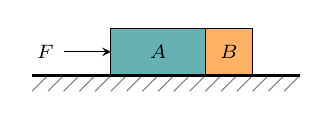
\begin{tikzpicture}[>=stealth,font=\scriptsize]
	\draw[fill=teal!60] (0,0) rectangle(1.2,0.6)node[midway]{\(A\)};
	\draw[fill=orange!60] (1.2,0) rectangle(1.8,.6)node[midway]{\(B\)};
	\draw[->] (-.6,.3)node[left]{\(F\)}--(0,.3);
	\foreach \x in {-1,-.8,...,2.2}
		\draw[gray] (\x,-.2)--++(.2,.2);
	\draw[thick] (-1,0)--(2.4,0);
\end{tikzpicture}